\documentclass[12pt]{article} 
\usepackage[margin=1in]{geometry} 
\usepackage{amsmath,amsthm,amssymb}
\usepackage{amsmath,amsfonts,amssymb,amsthm,epsfig,epstopdf,titling,url,array}
\usepackage{graphicx}
\begin{document}

\title{Comparative Analysis of the Large-Scale Structure of the Universe under Varying Assumptions}
\author{Mike Wu, Jessica Cisewski}

\maketitle
\section{Motivation}
The global structure of the Universe is thought to be composed of a distribution of matter and energy. By a large margin, dark energy is the most common element, thought to permeate all of space, contributing to as much as 68.3\% percent of the observable universe. Dark matter, a hypothetical form of matter that neither absorbs nor emits light, is thought to occupy a remaining 26.8\% of the observable universe, leaving baryonic matter, or ordinary matter such as the stars, planets, and humans, only 4.9\%. 

These definitions, while accepted by the majority of the cosmological community, are based heavily on assumptions. There is little evidence of dark matter existing as a particle, and researchers have not been able to create or consistently measure such a particle. Given that the only evidence for dark matter is observation of gravitational forces, there is a question of whether dark matter truly exists or if there are edge cases to our understanding of gravity.

Provided this uncertainty, one approach to gaining understanding of the true structure of the Universe is through cosmological simulations. Given the capacity to measure the observable universe, scientists have well-documented its current state. By changing the assumptions by which the simulations are built on, i.e. hydrodynamical forces, decoupling and cooling factors, cosmic wind speeds, one can find the set of initial conditions that best reflect the true Universe. However, in order to find the best initial conditions, one has to be able to compare different simulations. Simulations produce complex structures, and simple image analysis algorithms will not be able to distinguish finer details. To better make comparisons, an algorithm must exist that can locate a wide variety of objects in complex space.

\begin{figure}[!htb]
\minipage{0.25\textwidth}
  \centering
  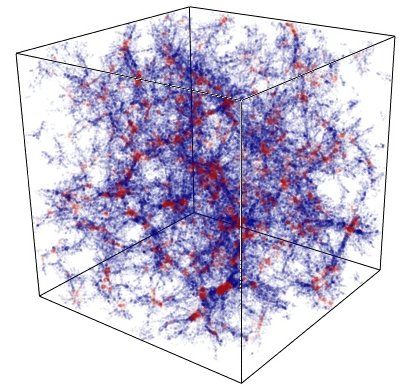
\includegraphics[width=0.9\linewidth]{LCDMstructure.jpg}
\endminipage\hfill
\minipage{0.25\textwidth}
  \centering
  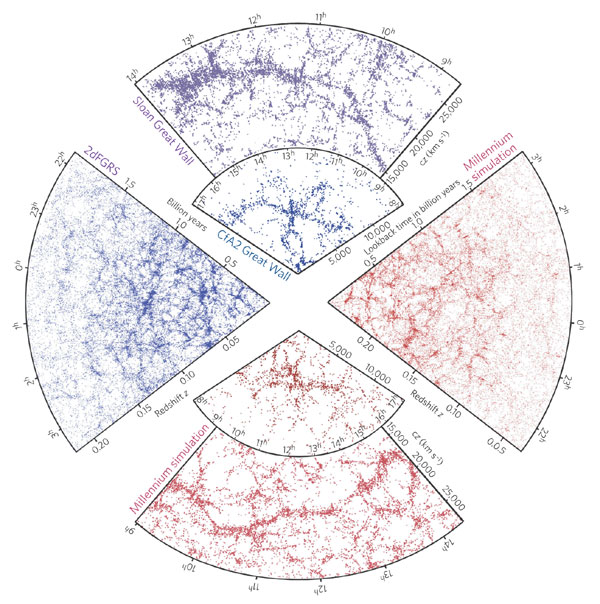
\includegraphics[width=0.9\linewidth]{nature04805-f1_2.jpg}
\endminipage\hfill
\minipage{0.50\textwidth}
  \centering
  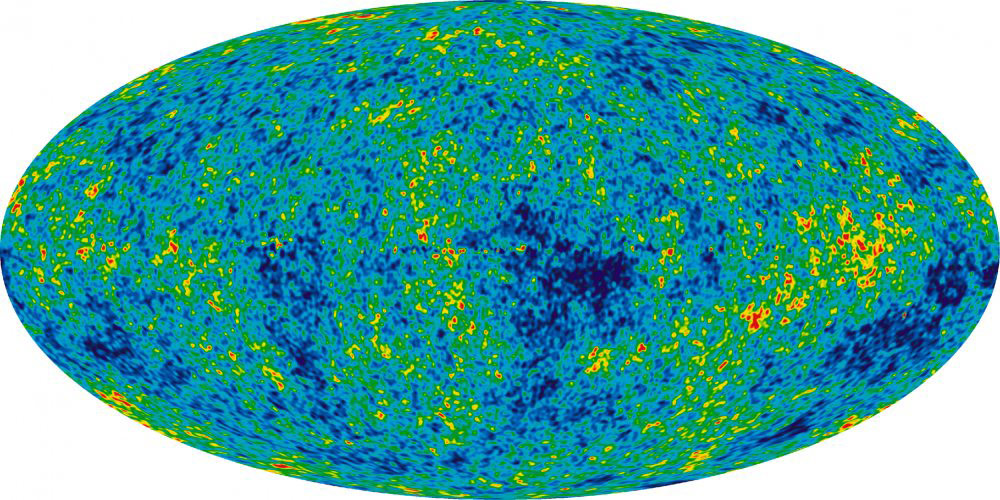
\includegraphics[width=0.8\linewidth]{simulation.jpg}
\endminipage\hfill
\caption{(Left) : A dark matter simulation cube of size 180 Mpc/h. Clusters are identified by the eigenvalues of the tidal field tensor and indicated by red colors. (Middle) : The galaxy distribution obtained from spectroscopic redshift surveys and from mock catalogues constructed from cosmological simulations. (Right) : The map of cosmic microwave background temperature fluctuations (European Space Agency Planck mission). }
\end{figure}

\section{Persistent Homology}

\section{Research Goals}
The goal of the research is to develop methods, possibly based on persistent homology, to compare probable realizations of the Universe under different sets of assumptions. Being able to appropriately analyze structure provides a standardized approach to quantitatively judge the similarities between pairs of universes. Doing so could lead to better approximations of the true initial conditions of the Universe and its development to the current state. 

Secondly, the ability to quantify structure may shed light on different properties and theories of dark matter. In theory, dark matter is divisible into hot and cold counterparts. Presuming that dark matter is a particle, hot dark matter particles are thought to move at ultrarelativistic speeds. For example, the neutrino, an electrically neutral elementary particle with half-integer spin, is considered hot dark matter and is unaffected by fundamental forces but measurable by a gravitational interaction. Conversely, cold dark matter particles move slowly. Due to its slow velocity, cold dark matter is thought to have higher probabilities of smaller objects collapsing and merging into larger hierarchical objects. Provided that, many physicists often attribute the transformation of the initial Universe from a smooth initial state to a lumpy distribution of galaxies and clusters to cold dark matter ($\lambda$CDM theory). A second research goal would be to analyze the structure of hot and cold dark matter simulations and draw conclusions on their differing physical and locational properties. 

\begin{figure}[!htb]
	\centering
    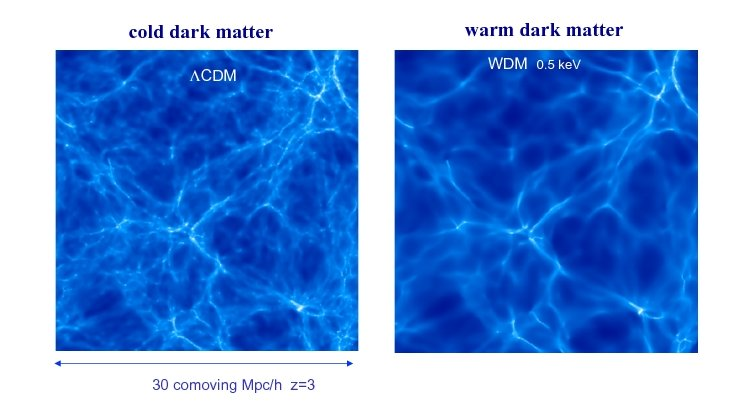
\includegraphics[width=0.5\linewidth]{simulations.jpg}
    \caption{A visual comparison between simulations of cold and hot/warm hard matter. The streaming motions of warm dark matter suppress structure formation on small scales.}
\end{figure}

All research material will be hosted in a public Github repository and all computational code will be written in R and Python. 

\end{document}


